\section{Wirtschaftsinformatik}

Der Forschungsbereich der Wirtschaftsinfomratik ist stark durch die beiden paradigmischen Anstäze der Gestaltungs- sowie Verhaltenorientierung geprägt. 
Die Wirtschaftsinformatik sieht sich selbst als interdisziplinare Realwissenschaft, welche Bereiche aus der technischen Perspektive als auch aus der betriebwissenschaftlichen Sichtweise betrachtet und beide verbindet.
Streng genommen weisen die Forschungskulturen der deutschen Wirtschaftsinformatik einerseits und der angloamerikanischen Schwesterdiszplin der Information Systems andererseits große Unterschiede hinsichtlich postulierter Methoden sowie Zielpräferenzen auf. Vor dem Hintergrund der in dieser Arbeit vorrangigen Untersuchung empirischer Evaluationsmethoden ist eine strikte Trennung beider Gebiete in dieser Hinsicht allerdings nicht zwingend notwendig.  Beide Disziplinen unterscheiden zwischen den sich gegenüberstehenden Forschungsparadigmen der Gestaltungsorientierung („Design Science“ im internationalen Raum) und der Erklärungsorientierung („Behaviroul Science“). Die deutsche WI sieht sich dabei stärker auf den praxisorientierteren Gestaltungsansatz fokussiert (Relevanz), wogegen ihr internationale Vertretung den theoretisch geprägten erklärungsorientierten Ansatz in den Vordergrund stellt (Rigor).  Die Ziele der Verhaltensorientierung sind vor allem die des Erklärens und Beschreibens von Zusammenhängen und Theorien (Wahrheitsfindung). Die Hauptfelder gestaltungsorientierter Wirtschaftsinformatik liegen hingegen in der Schaffung und Evaluierung zweckmäßiger Artefakte. Ziel von Design Science ist die Schaffung und Evaluierung zweckbezogener Artefakte zur Lösung von Organisationsproblemen (Simon?) {Frank 1999 69} Ziel dieser Artefakte ist es, bereits vorhandene Anwendungssysteme zu erweitern oder Probleme zu lösen, die entweder durch informationstechnische Anwendungen zuvor nicht zufriedenstellend gelöst wurden oder konnten. Die Gestaltungsorienteirete Forschung liefert dazu neue Lösungen als IT Artefakt, etwa in Form von Softwareprotytypen, deren Nutzen es im Prozess durch Anwendung geeigneter Forschungsmethoden zu evaluieren gilt. Dabei treten beide Forschungsparadigmen nicht streng dichotom auf, sondern können und müssen sich synergetisch ergänzen. Gerade im Zusammenhang mit dem langen geführten Diskurs zwischen Rigor und Relevanz zeigte sich, dass sich die deutsche Wirtschatfsinformatik zu stark auf den  \label{test}praxisnahen gestaltungsorientioerten Ansatz besinnte. Einerseits wird dieses Vorgehen von vielen Autoren gelobt (Momerndum für die gestatungsorientioere WInfo), andereseits wird auch oft das fehlende theoretische Fundament bemängelt. Gerade im Vergleich zur internationaen Wirtschaftsinformatik, welche sich stärker auf die theorethscihe fundierung bedacht ist, herrsche in der deutschen WI nachholbedarf. Auch die internationale Wi rief mit ihrer klaren Positionierung zur theoretischen Empirie zum Diskurs auf, sprach ihrerseits sogar von einer Identitäskrise (Benbasat und Zmud). Benbast und Zmud kritisierten diesen Fokus und verlangte danach, dass IT-Artefakt in den Mittelpunkt zu stellen und sich auf die Konstruktion nützlicher zu besinnen: Focus should be on how to best design IT artifacts and IS systems to increase their compatibility, usefulness, and ease of use or on how to best manage and support IT or IT-enabled business initiatives.
Das gemeinschaftliche Ziel der deutschen sowie internationalen Wirtschaftsinformatik besteht daher in der Sicherstellung und Steigerung der „Relevanz und Rigor“ Prämisse, also der praxisorientierten gestalterischen Artefaktentwicklung (Gestaltungsorientiert) sowie gleichzeitiger Korrektheit durch Prüfung mittles angemessener theoretischer Fundierung (Erklärungsorientiert). {Alturki 2012 32: 313} In Anbetracht dieses Ziels gilt es als Aufgabe der Wirtschaftsinfomratik das  richtige Verhältniss im Nutzen beider Forschungsansätze zu finden und implementieren. {Becker 2008 239: 5}

Der erforderliche Evaluationsschritt innerhalb der DesignScience versucht die Nützlichkeit eines Artefaktes zu „erklären“. Dieser Vorgang ist definitionsgemäß der Behavirolistischen Orientierung zuzuschreiben. Dadurch finden dessen verfügbaren Methoden implizit auch im Gestaltungsprozess Anwendung.  


In der Vergangenheit wurden eine Vielzahl möglicher Klassifikation von IT-Artefakten vorgenommen (Alter?) Die in diesem Zusammenhang jedoch meist genutze war die von HamrchSmith und Hevner dargestellte Unterschidung der Artefakte in: Konstrukte, Modelle, Methode, Instantiierung.
Bei der Definition eines IT-Artefaktes herrscht nach Alter kein kohärentes Verständnis über die genaue Definition eines IT-Atefaktes entwickelt hat, so sprechen sich viele für die von Simon postulierten Definition nach den Arten von Artefakte aus. Diese stellen sich demnachin Form von Konstrukten, Modellen, Methoden oder instatiierungen dar.
Nach Wotawa u. Thierau 1990 kennzeichnet sich die Evaluirung dieser Artefakte durch eine systematische Tätigkeit, welche eine Bewertung einer Sache (Artefakt) nach zweckgerichteter Form vornimmt. Somit dient die Artefaktevaluaiton vornehmlich der Feststellung jender „Nützlichkeit“.

Hess stellte diesen Vorgang schematisch wie in Fig 3 dargestellt auf:




\vspace{1cm}


\begin{mydef}{Wirtschaftsinformatik}{def_wi}
  Im Zuge dieser Arbeit impliziert der Begriff „Wirtschaftsinformatik“ die Betrachtung (konstruierter) IT-Artefakte ausschließlich in Form softwareseitiger Anwendungssysteme.
  This theorem is numbered with  \ref{def:def_wi} and is given on page \pageref{def:def_wi}.
\end{mydef}


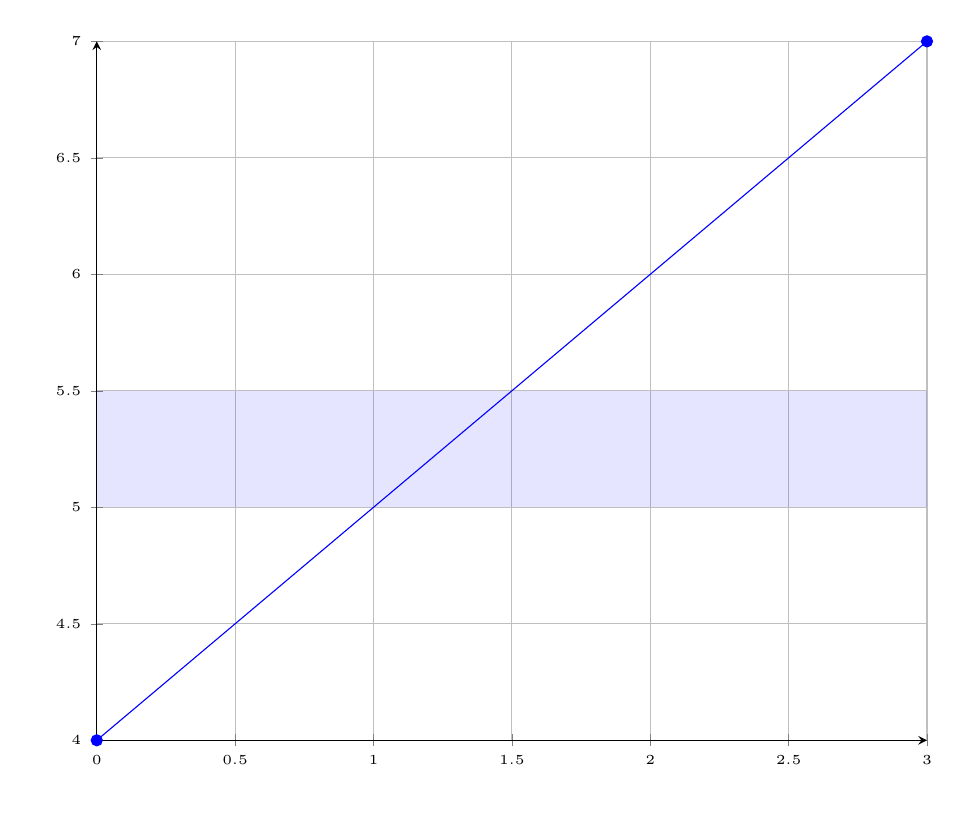
\begin{tikzpicture}
\begin{axis} [axis x line=bottom, axis y line = left, grid, width=\textwidth,
]
\addplot coordinates {(0,4) (3,7)};
\fill[blue, opacity=.1] (0,5) rectangle (3,5.5);
\end{axis}
\end{tikzpicture}

\begin{tikzpicture}
\begin{axis}
\addplot coordinates {(0,4) (3,7)};
\end{axis}
\end{tikzpicture}

 
\begin{figure}[h]
 \centering
 %\resizebox{\textwidth}{!}{%
 \IfFileExists{../../_preamble/check_file.tex}% prüfen aus welcher datei der aufruf stattfindet
{%
\providecommand{\myPath}{../../}% file exists=true: befinde mich im unterverzeichnis
}%
{%
\providecommand{\myPath}{}% file exists=false: befinde mich im root_verzeichnis
}%
\documentclass[tikz]{standalone}
%% läd standalone-klasse mit tikz-argument
%//Tikzbibliotheken\\%
\usetikzlibrary{						% Bibliotheken zur direkten Einbindung in TIKZEdt
arrows, 
fit,
shapes.geometric, 
matrix,
calc,
decorations.markings,
decorations.pathreplacing,
decorations.pathmorphing,
backgrounds,
shadings, 
shadows,
positioning,
mindmap,
trees,
datavisualization
}%% diverse tikz-bibliotheken
%%Font etc.%%
\usepackage{lmodern}					% OK, Latin Modern font,											check: 25.08.18
\usepackage{xcolor} 					% OK, Definieren und Nutzen von versch. Farben						check: 25.08.18
\usepackage{graphicx}					% OK, Bereitstellen von \includegraphics							check: 25.08.18

%%Forest%%
\usepackage{forest}						% OK, Baumdarstellung aus dem linguistischen Bereich				check: 25.08.18
\useforestlibrary{edges}

%%Venndiagramm%%
\usepackage{venndiagram}				% OK, Definieren und Darstellen von Venndiagrammen					check: 25.08.18

%%Tabellen%%
\usepackage{booktabs}					% OK, Schönere Tabellen ohne vertikale Linien \toprule etc.			check: 25.08.18
\usepackage{tabularx}					% OK, Weiterer Spaltentyp passt Tabellenbreite  automatisch an		check: 25.08.18
\usepackage{multirow}					% OK, Zellenspannung über mehrere Zeilen							check: 25.08.18
%\usepackage{makecell}					% OK, Tabellenlayout (Tabaellenheader) ähnlich \multirow			check: 25.08.18
\usepackage{tablefootnote}				% OK, Fußnoten in Tabellen (\footnote funktioniert nicht)			check: 25.08.18
\usepackage{array} 						% OK, Erstellen eigener Columntypen in Tabellenumgebungen			check: 25.08.18

%%Grafiken und Plots%%
\usepackage{tikz} 						% OK, Natives zeichnen in Latex ,									check: 25.08.18
\usepackage{tikz-cd} 					% OK, Erstellen von kommutativen Diagrammen in Tikz,				check: 25.08.18
\usepackage{pgfplots}					% OK, Plotten von Daten,											check: 25.08.18
\pgfplotsset{compat=newest}				% OK, Einstellen der Kompatibilitätsversion,						check: 25.08.18
\usepackage{pgfplotstable}				% OK, Plotten und schreiben von Daten in Tabellen,					check: 25.08.18
\usepackage{pgfcalendar} 				% OK, Umrechnen von Datumskoordinaten,								check: 25.08.18
\usepgfplotslibrary{dateplot}			% OK, Plotten von Datumskoordinaten,								check: 25.08.18
\usepgfplotslibrary{units}				% OK, Darstellen von Einheiten als Achsenlabel,						check: 25.08.18%% nur laden wenn weitere graphic pakete benötigt werden (tabellen, pgfplot,...)
%%define tikz-stlyes here, colours etc.
\tikzset{
block_phantom/.style={block_normal, draw=red, fill=none},
block_phantom/.style={block_normal, draw=blue, fill=none}
}
%\tikzstyle{block_phantom}=[block_normal, draw=red, fill=none]%% tikz-styles, farben etc.
\usepackage{pgfplots}
\usepackage{pgfplotstable}
\usepgfplotslibrary{dateplot}
\usepgfplotslibrary{units}
\usepackage{pgfcalendar} 
%%Kompatibilitäts-Version%%
\pgfplotsset{compat=newest}%% tikz-styles, farben etc.
\pgfplotsset{
  global_appearance/.style={
  grid_appearance,
  scale only axis,
  width= .75\textwidth,
  %width=12.5cm, % 13,5
  height=.4\textwidth
  }
}

\pgfplotsset{
  grid_appearance/.style={
   grid,
   grid style = {loosely dotted , thin},
  }
}

\pgfplotsset{
 %every axis plot/.append style={no markers},
  every pin/.append style={font=\footnotesize },
  every mark/.append style={scale=3},
  legend style=
  {
  font=\tiny, 
  %draw=none, 
  cells={align=left}, 
  at={(0.5,1.00)},
  anchor=north,
 % legend pos= north west
  },
  legend columns = 2,
  label style={font=\scriptsize},
  tick label style={font=\tiny},
}

\pgfplotsset{
  tuftle_like_axes/.style={
  thin,  %vorher semithick
  tick style={major tick length=4pt,thin,black}, %vorher semithick
  separate axis lines,
  axis x line*=bottom,
  axis x line shift=10pt,
  xlabel shift=5pt,
  axis y line*=left,
  axis y line shift=10pt,
  tick align = outside,
  ylabel shift=2pt,
  enlarge y limits=false,
  enlarge x limits=false,
  }
}

%%Tufte-Design%%
% \makeatletter
% \pgfplotsset{
  % tufte axes/.style =
    % {
      % after end axis/.code =
        % {
          % \draw ({rel axis cs:0,0} -| {axis cs:\pgfplots@data@xmin,0}) -- ({rel axis cs:0,0}  -| {axis cs:\pgfplots@data@xmax,0});
          % \draw ({rel axis cs:0,0} |- {axis cs:0,\pgfplots@data@ymin}) -- ({rel axis cs:0,0}  |-{axis cs:0,\pgfplots@data@ymax});
        % },
      % axis line style = {draw = none},
      % tick align      = outside,
      % tick pos        = left
    % }
% }
% \makeatother%% tikz-styles, farben etc.
\begin{document}%
\IfFileExists{../../_preamble/check_file.tex}% prüfen aus welcher datei der aufruf stattfindet
{%file exists=true: befinde mich im unterverzeichnis
\IfFileExists{data/check_file.tex}% aus welcher datei der aufruf stattfindet
 	{\pgfplotstableread[]{data/plot_gm_gmi.dat}\data}
 	{\pgfplotstableread[]{_img/_pgfplot/data/plot_gm_gmi.dat}\data}
% add new column with Julian integer numbers
% therefore a counter is needed
    \newcount\julianday
    \pgfplotstablecreatecol[
        create col/assign/.code={
            % convert the number of the current row and save it to `\julianday'
            \pgfcalendardatetojulian{\thisrow{year}}{\julianday}
            % then give the entry of `\julianday' to `\entry' which is then
            % given to the current cell
            \edef\entry{\the\julianday}
            \pgfkeyslet{/pgfplots/table/create col/next content}\entry
        },
    ]{JulianDay}{\data}
    % because the `dateplot' library shifts automatically all dates to 0 using
    % the first found coordinate we can't use the created `JulianDay' data
    % directly for `linear regression', but have to do the same first with
    % the data
        % get the first coordinate of the column ...
        \pgfplotstablegetelem{0}{JulianDay}\of{\data}
        % ... and store it in `\xmin'
        \pgfmathtruncatemacro{\xmin}{\pgfplotsretval}
    % now create another column with the shifted values
    \pgfplotstablecreatecol[
        expr={\thisrow{JulianDay}-\xmin},
    ]{JulianDayMod}{\data}

\begin{tikzpicture}
\begin{axis} [ 
width=\textwidth,
date coordinates in = x,
date ZERO = 1972-01-01,
xmin = 1980-01-01,
xmax = 2015-01-01,
%xtick distance=10,
%try min ticks = 5,
xticklabel=\year,
global_appearance,
tuftle_like_axes,
xlabel={},
ylabel={Anzahl Ver\"offentlichungen [St\"uck]},
%xtick={data},
 xtick={
%1972-01-01, 
%1974-01-01, 
1976-01-01, 
%1978-01-01, 
1980-01-01, 
%1982-01-01,
1984-01-01,
%1986-01-01,
1988-01-01,
%1990-01-01,
1992-01-01,
%1994-01-01,
1996-01-01,
%1998-01-01,
2000-01-01,
2001-01-01,
2002-01-01,
2003-01-01,
2004-01-01,
2005-01-01,
2006-01-01,
2007-01-01,
2008-01-01,
2009-01-01,
2010-01-01,
2011-01-01,
2012-01-01,
2013-01-01,
2014-01-01,
2015-01-01},
%ytick={-50, 0, 200, 400, 600, 800},
ymin=0,
ymax=830,
x tick label style={rotate=45,anchor=north east}
% x unit=\si{},
 %y unit=\si{},
]
\IfFileExists{data/check_file.tex}% aus welcher datei der aufruf stattfindet
{%
\addplot [thin]table [x=year, y=gm]{data/plot_gm_gmi.dat};%
\addplot [densely dashed,  thin ]table [x=year, y=gmi]{data/plot_gm_gmi.dat};%
}%
{%
\addplot [thin]table [x=year, y=gm]{_img/_pgfplot/data/plot_gm_gmi.dat};%
\addplot [densely dashed, thin ]table [x=year, y=gmi]{_img/_pgfplot/data/plot_gm_gmi.dat};%
}%

\addplot[black, opacity=1, very thin,mark=halfsquare right*, mark options={color=black, scale=1}] table [x=year,y={create col/linear regression={x=JulianDayMod,y=gm}}]{\data};%%Regressionslinie
\addplot[black, opacity=1, very thin, mark=halfsquare left*,mark options={color=black, scale=1}] table [x=year,y={create col/linear regression={x=JulianDayMod,y=gmi}}]{\data};%%Regressionslinie

\addlegendentry{Gesch\"aftsmodell};
\addlegendentry{Gesch\"aftsmodell-\\innovation};
\addlegendentry{Regression GM};
\addlegendentry{Regression GMI};
%\node [pin=90: \footnotesize Regression Gesch\"aftsmodell] at (2000-01-01,255) {};
%\node [pin=-90: \footnotesize Regression Gesch\"aftsmodellinnovation] at (2011-01-01,105) {};
%\fill[blue, opacity=.1] (1984-01-01,6) rectangle (2015-01-01,800);
%\fill[blue, opacity=.1] (1984-01-01,0) rectangle (2015-01-01,200);
%\draw[black, opacity=1] (1984-01-01,0) to (2015-01-01,200);
%\draw[black, opacity=1, densely dashdotted] (1984-01-01,6) to (2015-01-01,800);
\end{axis}%
\end{tikzpicture}%
%
}%
{%file exists=false: befinde mich im root_verzeichnis
\IfFileExists{data/check_file.tex}% aus welcher datei der aufruf stattfindet
 	{\pgfplotstableread[]{data/plot_gm_gmi.dat}\data}
 	{\pgfplotstableread[]{_img/_pgfplot/data/plot_gm_gmi.dat}\data}
% add new column with Julian integer numbers
% therefore a counter is needed
    \newcount\julianday
    \pgfplotstablecreatecol[
        create col/assign/.code={
            % convert the number of the current row and save it to `\julianday'
            \pgfcalendardatetojulian{\thisrow{year}}{\julianday}
            % then give the entry of `\julianday' to `\entry' which is then
            % given to the current cell
            \edef\entry{\the\julianday}
            \pgfkeyslet{/pgfplots/table/create col/next content}\entry
        },
    ]{JulianDay}{\data}
    % because the `dateplot' library shifts automatically all dates to 0 using
    % the first found coordinate we can't use the created `JulianDay' data
    % directly for `linear regression', but have to do the same first with
    % the data
        % get the first coordinate of the column ...
        \pgfplotstablegetelem{0}{JulianDay}\of{\data}
        % ... and store it in `\xmin'
        \pgfmathtruncatemacro{\xmin}{\pgfplotsretval}
    % now create another column with the shifted values
    \pgfplotstablecreatecol[
        expr={\thisrow{JulianDay}-\xmin},
    ]{JulianDayMod}{\data}

\begin{tikzpicture}
\begin{axis} [ 
width=\textwidth,
date coordinates in = x,
date ZERO = 1972-01-01,
xmin = 1980-01-01,
xmax = 2015-01-01,
%xtick distance=10,
%try min ticks = 5,
xticklabel=\year,
global_appearance,
tuftle_like_axes,
xlabel={},
ylabel={Anzahl Ver\"offentlichungen [St\"uck]},
%xtick={data},
 xtick={
%1972-01-01, 
%1974-01-01, 
1976-01-01, 
%1978-01-01, 
1980-01-01, 
%1982-01-01,
1984-01-01,
%1986-01-01,
1988-01-01,
%1990-01-01,
1992-01-01,
%1994-01-01,
1996-01-01,
%1998-01-01,
2000-01-01,
2001-01-01,
2002-01-01,
2003-01-01,
2004-01-01,
2005-01-01,
2006-01-01,
2007-01-01,
2008-01-01,
2009-01-01,
2010-01-01,
2011-01-01,
2012-01-01,
2013-01-01,
2014-01-01,
2015-01-01},
%ytick={-50, 0, 200, 400, 600, 800},
ymin=0,
ymax=830,
x tick label style={rotate=45,anchor=north east}
% x unit=\si{},
 %y unit=\si{},
]
\IfFileExists{data/check_file.tex}% aus welcher datei der aufruf stattfindet
{%
\addplot [thin]table [x=year, y=gm]{data/plot_gm_gmi.dat};%
\addplot [densely dashed,  thin ]table [x=year, y=gmi]{data/plot_gm_gmi.dat};%
}%
{%
\addplot [thin]table [x=year, y=gm]{_img/_pgfplot/data/plot_gm_gmi.dat};%
\addplot [densely dashed, thin ]table [x=year, y=gmi]{_img/_pgfplot/data/plot_gm_gmi.dat};%
}%

\addplot[black, opacity=1, very thin,mark=halfsquare right*, mark options={color=black, scale=1}] table [x=year,y={create col/linear regression={x=JulianDayMod,y=gm}}]{\data};%%Regressionslinie
\addplot[black, opacity=1, very thin, mark=halfsquare left*,mark options={color=black, scale=1}] table [x=year,y={create col/linear regression={x=JulianDayMod,y=gmi}}]{\data};%%Regressionslinie

\addlegendentry{Gesch\"aftsmodell};
\addlegendentry{Gesch\"aftsmodell-\\innovation};
\addlegendentry{Regression GM};
\addlegendentry{Regression GMI};
%\node [pin=90: \footnotesize Regression Gesch\"aftsmodell] at (2000-01-01,255) {};
%\node [pin=-90: \footnotesize Regression Gesch\"aftsmodellinnovation] at (2011-01-01,105) {};
%\fill[blue, opacity=.1] (1984-01-01,6) rectangle (2015-01-01,800);
%\fill[blue, opacity=.1] (1984-01-01,0) rectangle (2015-01-01,200);
%\draw[black, opacity=1] (1984-01-01,0) to (2015-01-01,200);
%\draw[black, opacity=1, densely dashdotted] (1984-01-01,6) to (2015-01-01,800);
\end{axis}%
\end{tikzpicture}%
\\%\\
%\begin{tikzpicture}
\begin{axis}[
ybar interval,
global_appearance,
tuftle_like_axes,
ymax=800,
ymin=0, 
ybar interval=1, 
date coordinates in = x,  
date ZERO = 1988-01-01, 
xmax = 2014-12-31, 
x tick label style={rotate=90,anchor=east},
%minor y tick num = 5,
ylabel = Anzahl Veröffentlichungen,
xticklabel=\year,
height=\axisdefaultheight,
]

\IfFileExists{data/check_file.tex}% aus welcher datei der aufruf stattfindet
{%
\addplot [thin]table [x=year, y=gm]{data/plot_gm_gmi.dat};%
\addplot [densely dashed,  thin ]table [x=year, y=gmi]{data/plot_gm_gmi.dat};%
}%
{%
\addplot [thin]table [x=year, y=gm]{_img/_pgfplot/data/plot_gm_gmi.dat};%
\addplot [densely dashed, thin ]table [x=year, y=gmi]{_img/_pgfplot/data/plot_gm_gmi.dat};%
}%
\end{axis}
\end{tikzpicture}%\\
}%
\end{document}%
%
 %}
 \caption{}
 \end{figure}
 
 
